\chapter{Trabalho Proposto} \label{cap:tp}
%2345678901234567890123456789012345678901234567890123456789012345678901234567890

O trabalho visa o desenvolvimento de uma ontologia que englobe o modelo
psicológico de emoções explicado na seção~\ref{cap:eda:mce}, uma ontologia de
humanos virtuais e de características. Cada ontologia à ser explicada foi pensada
como um modulo que pode ser usada em separado dos demais. A criação das mesmas
tem como vantagens fazerem o raciocínio e a definição de um vocabulário
básico. Dessa forma, o tempo de aprendizado tende a ser menor e a baixar o
tempo de configuração.

O presente capítulo foi dividido em partes. A primeira, descreve a ontologia
afetiva desenvolvida se baseando em um modelo da psicologia. A descrição de
como a ontologia de humanos virtuais foi reutilizada esta explicada na
seção~\ref{cap:tp:ruodhv}. Na \ref{cap:tp:odp}, a ontologia de característica é
detalhada. Por fim, a última demostra a utilização das mesmas.
%\ref{cap:tp:cdu}

\section{Ontologia Afetiva} \label{cap:tp:oa}

A fundamentação do modelo afetivo sendo utilizado aqui é o proposto por
\citet{ortony1988cse} e encontra-se explicado na seção \ref{cap:eda:mce}. A
ontologia proposta tinha como ideia inicial não utilizar regras, porém como
pode ser observado na Tabela~\ref{tab:oa:geral} foi necessário a criação de
regras para suportar o raciocínio no nível de indivíduo corretamente. As
regras que ajudam a conclusão das relações \emph{hasKnow}, \emph{hasFriend} e
\emph{hasEnemy} são diferentes das demais por causa que elas tem como
característica operar no domínio e na imagem da classe \emph{Agent}. Por
exemplo, se John avalia que se relaciona bem com Jose então John
\emph{hasFriend} Jose. Note que o contrario não é necessariamente verdade, o
Jose pode apenas saber que conhece o John então Jose \emph{hasKnow} John.

\begin{table}
	\caption{Ontologia proposta com expressividade: ALCHIN(D).}
	\label{tab:oa:geral}
	\begin{center}
	\begin{tabular}{|c|c|}
	%\begin{tabular}{|p{34mm}|p{50mm}|p{50mm}|}
		\hline
		Descrição & Quantidade \\ \hline
		Classes &  45 		\\ \hline
		Propriedade de Objetos & 16 \\ \hline
		Propriedade de Dados & 14 \\ \hline
		Indivíduos &  0		\\ \hline
		Regras & 7 \\ \hline
	\end{tabular}
	\end{center}
\end{table}

Na Figura~\ref{fig:rlocc} são mostradas as regras desenvolvidas, elas dependem
que os indivíduos da ontologia sejam marcados como diferentes um do outro.
Assim, recomenda-se fortemente que quando registrar um indivíduo da classe
\emph{Object} ou \emph{Agent} que a informação de igualdade ou diferenciação
seja preenchida\dev{}. Assim, se evita que o raciocinador conclua que não
conhece a resposta e chegue a uma conclusão não esperada.

\begin{figure}[t]
  \centering
  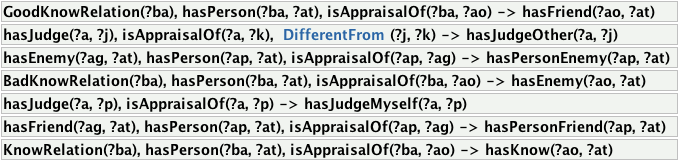
\includegraphics[width=14cm]{figuras/rules-LOCC.png}
  \caption{Regras da ontologia proposta.}
  \label{fig:rlocc}
\end{figure}

A Figura~\ref{fig:kplocc} mostra a árvore de relações que tem como imagem
dados ou instâncias (objetos). Ao se comparar as Figuras~\ref{fig:rlocc}
e \ref{fig:kplocc} se chega a conclusão que as propriedades que as
regras concluem não precisam ser configuradas pelo usuário. Assim, ao invés de
16 propriedades de objetos conforme informado na Tabela~\ref{tab:oa:geral}
apenas 9 precisam ser conhecidas. Dessas a propriedade mais utilizada é a
\emph{hasSomething} que serve para indicar o que esta sendo avaliado. Note que
\emph{hasPerson} deve ser usado quando o indivíduo em avaliação for um membro
da classe \emph{Agent}. Já, a relação \emph{hasJudge} serve para indicar que o
membro da classe \emph{Object} esta sendo avaliado. Por exemplo, Millie tem
uma avaliação julgando seu carro com uma valoração positiva.

\begin{figure}[b]
  \centering
  \begin{tabular}{cc}
  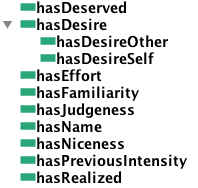
\includegraphics[height=4cm]{figuras/dataProperty-LOCC.png} & 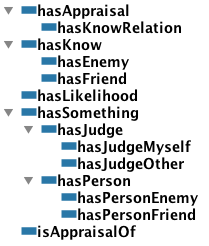
\includegraphics[height=5cm]{figuras/objectProperty-LOCC.png} \\
  (i) Relações de dados & (ii) Relações de Objetos
  \end{tabular}
  \caption{As relações existentes na ontologia proposta.}
  \label{fig:kplocc}
\end{figure}

Todos os dados numéricos da ontologia são inteiros. Isso foi feito com a
finalidade de permitir que o usuário normalize\dev{} o número obtido da
maneira que desejar. Além disso, foi tomada a decisão de não especificar o
domínio da maioria das propriedades por causa que isso forçaria um
enquadramento em classes não desejadas. Por exemplo, se a relação
\emph{hasLikelihood} tiver o domínio \emph{ConsequenceForSelf} e existir
indivíduo com somente essa relação então o mesmo seria enquadrado no conceito
\emph{ConsequenceForSelf}. O correto nesse caso seria não ser concluído nada,
isto é, pertencer à classe \emph{Thing}.

A estrutura da ontologia pode ser visualizada na Figura~\ref{fig:tlocc}. Além
disso, pode ser recomendável olhar a
Figura~\ref{fig:occ_model}~(pg.~\pageref{fig:occ_model}) do modelo criado por
\citet{ortony1988cse} durante o resto da discussão dessa seção. Os
sub-conceitos de \emph{Emotion} correspondem aos ramos do modelo \occ original.
O ramo \emph{ActionsOfAgents} julga a responsabilidade e o quanto o agente que
realizou uma ação ou evento se desviou do esperado, o de
\emph{ConsequencesOfEvents} julga a consequência de um evento e
\emph{AspectsOfObjects} julga a atração para com um objeto.

O primeiro ramo a ser abordado é, o menos cognitivo, \emph{AspectsOfObjects}.
As emoções desse tipo são relacionadas com atratividade e familiaridade.
Entretanto, essas duas relações foram consideradas equivalentes porque o
importante, para o modelo, é quando ambas são positivas ou ambas negativas.
Assim sendo, uma pode assumir os dois papeis sem maiores penalidades e
simplificando a modelagem. A emoção \emph{Hate} é modelada como tendo a
propriedade de familiaridade (\emph{hasFamiliarity}) com valores negativos,
enquanto a emoção \emph{Love} tem valoração dessa mesma propriedade positiva.
Caso o valor seja zero, nada pode ser concluído.

\begin{wrapfigure}{r}{0.4\textwidth}
  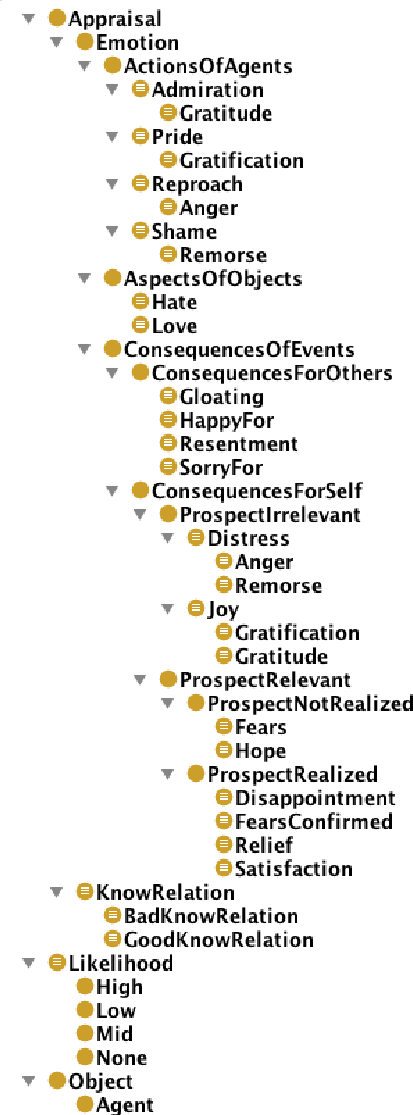
\includegraphics[height=16cm]{figuras/hierarquiaLOCC.png}
  \caption{Taxonomia da ontologia proposta baseado no modelo.}
  \label{fig:tlocc}
\end{wrapfigure}

Cabe notar que parece estranho uma emoção \emph{Love} com um objeto, porém
essa emoção foi escolhida por quem montou o modelo por ser a emoção mais forte
de seu tipo. Assim, níveis menores implicam em outros tipos de emoção. Além
disso, conforme explicado no trabalho, agentes podem ser vistos como objetos
quando se esta avaliando a sua atração. Assim, todo agente (\emph{Agent}) é um
objeto (\emph{Object}). Por exemplo, John esta apaixonado pela Millie ou
John tem repulsa por televisão.

O segundo conceito, chamado \emph{ActionsOfAgents}, pode ser pensado como
um ramo que julga a responsabilidade por uma determinada ação ou evento.
Assim, esse ramo é capaz de gerar emoções de: Admiração (\emph{Admiration}),
Orgulho (\emph{Pride}), Vergonha (\emph{Shame}) e Reprovação
(\emph{Reproach}). Por exemplo, Jose possui orgulho por cozinhar ou Dilu
reprova Jose porque ele come carne.

Na definição, as emoções de orgulho e vergonha podem acontecer mesmo quando se
esta avaliando ações de outras pessoas. Por exemplo, Dolores tem vergonha de
sua mãe que não cozinha. Essa conclusão é possível por causa de uma relação
que eles propõem de empatia. Entretanto, como em nenhum outro momento, eles
dão mais detalhes sobre essa empatia foi resolvido considerar que vergonha e
orgulho são emoções sentidas somente quando o agente esta avaliando a si mesmo
e, dessa forma, o exemplo anterior não é possível. \dev{}
% dev -> poderia ter sido usado float e ter feito 1 (para si) e 0 (para outro)

As emoções que julgam responsabilidade são definidas como tendo uma relação de
julgamento (\emph{hasJudge}) e uma relação que mapeia o valor do julgamento
(\emph{hasJudgeness}) que representa o quanto o agente se desviou do
comportamento esperado, isto é, em casos de aprovação é um valor positivo e em
casos de reprovação é um valor negativo. Todavia, isso ainda não permite
diferenciar a emoção de admiração da emoção de orgulho ou a reprovação da de
vergonha. Essa distinção é possível ao se dividir a relação de julgamento com
duas sub-relações: tem auto-julgamento (\emph{hasJudgeMyself}) e tem
julgamento de outro (\emph{hasJudgeOther}).

A utilização de sub-propriedade torna possível escrever a ontologia da maneira
esperada suprimindo o problema. Entretanto, para o usuário pode se tornar
complicado ter que lembrar quando utilizar uma sub-propriedade ou outra.
Assim, foi resolvido deixar o usuário sempre utilizar a relação de julgamento
(\emph{hasJudge}) e via 2 regras inferir se é um auto-julgamento ou o
julgamento de outra pessoa. Para essas regras funcionarem da maneira correta,
o usuário deve declarar que os agentes ou objetos são diferentes. Caso isso
não ocorra, o sistema considera que não há informação para verificar se um
individuo é igual ou diferente que o outro e concluir que não conhece a
resposta. Além disso, a relação de julgamento tem como imagem o conceito
\emph{Object}. Dessa forma, os exemplos anteriores são todos válidos.

Cabe salientar que toda avaliação tem pelo menos duas relações. A primeira
relação serve para conhecer quem esta avaliando (\emph{isAppraisalOf}) e a
outra serve para indicar quem ou o que esta sendo avaliado
(\emph{hasSomething}). Em muitas avaliações essa última pode não ser
informada sem nenhum prejuízo. O último ramo, chamado de
\emph{ConsequencesOfEvents} é dividido em: \emph{ConsequencesForSelf} e
\emph{ConsequencesForOthers}. Toda essa divisão foca na consequência de um
evento ou ação realizado por um determinado agente. Por exemplo, Dilu tem pena
de Jose, Jose tem esperança de ser promovido, John tem satisfação por
estar almoçando ou Millie esta alegre por cozinhar.

A \emph{ConsequencesForOthers} expressa 4 emoções: \emph{HappyFor},
\emph{SorryFor}, \emph{Gloating} e \emph{Resentment}. Na definição, essas
emoções dependem: do grau de desejabilidade do avaliador para com o outro; do
grau de desejabilidade que se presume que o outro tenha; do grau de
merecimento do evento; do tipo de relacionamento com a pessoa. Na ontologia
proposta, a principal diferença com o modelo original é que foi considerado
que o grau de desejabilidade do avaliador para com o outro e o grau de
merecimento do evento são os mesmos. Dessa forma, se pode utilizar apenas três
relações para descrever as 4 emoções.

A relação de merecimento (\emph{hasDeserved}) e relação de desejabilidade
presumida (\emph{hasDesireOther}) são avaliadas de acordo com sua valoração
positiva ou negativa. A relação \emph{hasPerson} liga o outro individuo
sendo avaliado com a avaliação. Para se ter o conhecimento de quem esta
julgando é uma pessoa amiga (\emph{GoodKnowRelation}) ou inimiga
(\emph{BadKnowRelation}), esses conceitos foram criados e precisam ser
configurados para cada um dos agentes em questão. O agente pode declarar que
só conhece uma pessoa, que conhece e é um amigo ou que conhece e não gosta
dela (inimiga). Entretanto, quem precisa dessa informação é o conceito de
avaliação quando as relações \emph{hasPersonEnemy} e \emph{hasPersonFriend}
precisam ser descobertas.

\emph{ConsequencesForSelf} se divide entre consequências de eventos com
probabilidade relevante (\emph{ProspectRelevant}) e irrelevante
(\emph{ProspectIrrelevant}). Cabe salientar que esses dois conceitos se
relacionam com probabilidade (\emph{hasLikelihood}), entretanto enquanto o
primeiro conceito se relaciona com a parte não nula. A outra se relaciona
somente com essa. Dessa forma, ambos os conceitos são disjuntos. A classe de
probabilidade relevante pode ser dividida ainda entre possibilidade não
realizada (\emph{ProspectNotRealized}) e realizada (\emph{ProspectRealized}).

As emoções \emph{Hope} e \emph{Fear} fazem parte do conceito
\emph{ProspectNotRealized}. Esse conceito usa as relações \emph{hasLikelihood}
e \emph{hasDesireSelf}. Essa última propriedade é um número que
representa o desejo de se obter ou repudiar o evento. Além disso, quando o
evento ocorre a emoção atual pode virar uma emoção do conceito
\emph{ProspectRealized}, isto é, \emph{Fear} pode virar ou
\emph{FearsConfirmed} ou \emph{Relief} e \emph{Hope} pode virar ou
\emph{Satisfaction} ou \emph{Disappointment}.

O conceito \emph{ProspectRealized} não se relaciona em nenhum momento com a
relação \emph{hasLikelihood} porque o evento já aconteceu ou não vai mais
acontecer. Assim, ele possui três relações distintas das anteriores, a
primeira é o grau de realização de um evento (\emph{hasRealized}), isto é, a
visão do agente sobre como a consequência do evento aconteceu. A segunda
relação \emph{hasPreviousIntensity} recebe a valoração da emoção de medo ou
esperança do evento que tinha probabilidade e serve para saber se o evento era
um evento bom (esperança) ou ruim (medo). Já, a terceira \emph{hasEffort}
tenta estimar o grau de esforço que foi dispendido para a atração ou repulsa
da consequência do evento.

O conceito \emph{ProspectIrrelevant} é parecido com o conceito
\emph{ProspectRelevant} com a diferença que a relação \emph{hasLikelihood} vai
somente para valores nulos. Alem disso, as emoções desse conceito e do
\emph{ActionsOfAgents} podem ser misturadas formando conceitos compostos.
A composição é quando uma emoção pode ser encaixada em mais de uma emoção
como no caso de se estar alegre (\emph{Joy}), orgulhoso (\emph{Pride}) e
gratificado (\emph{Gratification}). Por fim, o conceito \emph{Setup}
\todo{na dissertacao falar mais sobre isso} é o utilizado para manter junto da
ontologia criada o limite mínimo para uma emoção virar sentimento\dev{}.

%a transferencia eh feita pelo sistema;
%os dados sao carregados para memoria e eliminados;
%conforme reparado nao ha decaimento da emocao, a mesma eh instantanea;
%2345678901234567890123456789012345678901234567890123456789012345678901234567890

\section{Reutilizando uma Ontologia de Humanos Virtuais} \label{cap:tp:ruodhv}

Na seção~\ref{cap:eda:odhv} foi explicado a ontologia de
\citet{Gutierrez:2007:OVH:1229160.1229164} que descreve humanos virtuais de
uma maneira bem detalhada. Entretanto, a intenção no presente trabalho é
focar no comportamento do personagem. Dessa forma, a ontologia que será
utilizada é a de \citet{paiva2005ontology} que descreve uma vida normal.

\begin{figure}[t]
  \centering
    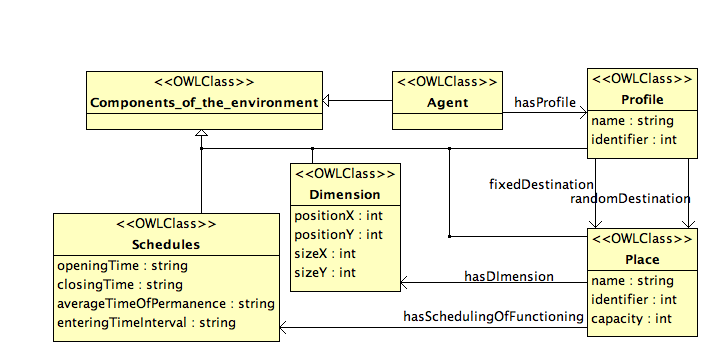
\includegraphics[width=150mm]{figuras/uem-tbox.png}
  \caption{T-Box baseado no modelo de ambiente urbano \cite{paiva2005ontology}.}
  \label{fig:UEM:TBOX}
\end{figure}

A Figura~\ref{fig:UEM:TBOX} demostra a ontologia que será utilizada, como é
possível observar as subclasses dos conceitos \emph{Profile} e \emph{Place}
foram removidas\footnote{Compare a Figura~\ref{fig:UEM:TBOX} com a
Figura~\ref{fig:UEM} da página~\pageref{fig:UEM}.} por serem consideradas parte
da A-Box. Além disso, o conceito \emph{Components\_of\_the\_environments} esta
sendo pensando como um sub-conceito do conceito \emph{Setup} na ontologia
desenvolvida por causa que esse representa configurações gerais.

%Essas configurações gerais são carregadas, normalmente, em outras partes do
%sistemas e então eliminadas por causa que elas não influenciam as emoções
%diretamente.
\todo{comentado porque por agora nao tem sistema nenhum, na dissertacao pd ir}
Fora isso, foi introduzido uma nova relação chamada \emph{hasCharacter} que
mapeia o conceito de agente da seção anterior para o conceito utilizado no
trabalho de \citet{paiva2005ontology}. Dessa forma, um agente na ontologia do
modelo \occ pode descobrir seu perfil e descobrir seus locais visitados
regularmente. Da mesma forma, o conceito de \emph{Place} faz uso da relação
\emph{hasSetup} porque os locais podem ser pensados como ``objetos
inteligentes'' dado que possuem horário de abertura e fechamento das
atividades.


% eu nao tenho certeza sobre isso, porem seria interessante ter uma relacao
% hasDimension da Object para Dimension. Dessa forma um objeto teria
% conhecimento mesmo que abstrato sobre suas dimensões para o caso de ser
% necessario fazer a bounding box collission...

\section{Ontologia de Características} \label{cap:tp:odp}
% de percepcoes virou do ambiente
% voltou a ser de percepcoes
% e agora virou caracteristicas hehehehe!

\citet{doyle1998annotated} propuseram que o mundo contivesse uma serie de
anotações nos objetos. Assim, o agente poderia conhecer apenas a forma de
questionar os objetos sobre suas formas de usar, suas descrições e suas outras
características. Esse conceito veio do conceito \emph{affordance} que se
refere a propriedade de um objeto que dita como o mesmo será utilizado.
Dessa forma, uma cadeira tem a propriedade de ser sentada e uma porta tem as
propriedades de ser aberta ou ser fechada.

Nesse trabalho foi usado 5 tipos de anotações: (i) anotações emocionais,
explicam como um agente responde ``emocionalmente''; (ii) anotações de
resposta, explicam como o agente deve reagir ao evento no ambiente pode ser
uma ação especifica ou uma sugestão de crença; (iii) anotações de resolução de
problemas, descreve o estado do problema  e permite anotar dicas que o agente
talvez fale ou realize; (iv) anotações de papel, informam o agente sobre ações
relevantes para determinados trabalhos no mundo; (v) anotações de jogo,
descreve o estado do jogo permitindo sugerir movimentos.

\citet{kallmann1999modeling} explicaram uma ideia similar, os objetos no mundo
são os responsáveis por proverem para o personagem o como ele deve ser usado.
Durante a animação do personagem estar abrindo a porta, por exemplo, quem esta
no controle do mesmo é o ``agente'' que controla a porta porque o agente do
personagem delega para o da porta realizar a sua animação. Dessa forma,
esses objetos inteligentes precisam ter um determinado nível de conhecimento
sobre o personagem.

De uma maneira similar, o conceito de artefatos que possuem propriedades
observáveis e utilizáveis foi criado por \citet{ricci31cartago}. Por exemplo,
uma porta pode ter como propriedade observável seu estado (estar aberta ou
estar fechada) e ação possível ou propriedade utilizável ser aberta ou ser
fechada. Essas ações podem ficar disponíveis conforme o estado atual do
objeto, mas o controle da disponibilidade é do próprio objeto por que é ele
que sabe como realizar a ação propriamente dita. O agente unicamente diz de
alguma forma que o objeto tem que realizar tal ação. Nesse trabalho, não é
mencionado que o agente pode ser temporariamente controlado por objetos.

Assim, a foi criado dois conceitos principais \emph{Annotation} e
\emph{Preference}. O conceito \emph{Annotation} é utilizado para representar
características de determinadas coisas. Essas características podem ainda
ser categorizadas entre as que mudam e não mudam durante a simulação. O
sub-conceito \emph{Dynamic} representa as características dinâmicas, isto é,
as características que podem ser alterados durante a ``vida'' do objeto. O
sub-conceito \emph{Static} representa as características que não podem ser
alteradas depois da criação do objeto. O calor e o dono são exemplos de
características dinâmicas, enquanto o nome e a capacidade são exemplos de
características estáticas.

A representação de preferência por determinadas características é representado
no conceito \emph{Preference}. A preferência representa como uma entidade ou
agente é atraído por determinada característica, por exemplo algumas pessoas
gostam de calor e outras não. Assim, as pessoas que gostam de calor são
atraídas pela valoração positiva da anotação de calor. Já, as pessoas que não
gostam de calor são atraídas pela valoração negativa. Dessa forma, os
sub-conceitos da preferência representam sempre valores que fazem o agente ser
atraído pelo objeto e repelido em caso contrário.

\section{Caso de uso} \label{cap:tp:cdu}

\begin{table}[b]
	\caption{As três ontologias juntas possuem expressividade: ALCHIN(D).}
	\label{tab:tp:cdu:geral}
	\begin{center}
	\begin{tabular}{|c|c|}
	%\begin{tabular}{|p{34mm}|p{50mm}|p{50mm}|}
		\hline
		Descrição & Quantidade \\ \hline
		Classes &  57 		\\ \hline
		Propriedade de Objetos & 23 \\ \hline
		Propriedade de Dados & 25 \\ \hline
		Indivíduos &  27	\\ \hline
		Regras & 7 \\ \hline
	\end{tabular}
	\end{center}
\end{table}

\begin{wrapfigure}{r}{0.38\textwidth}
  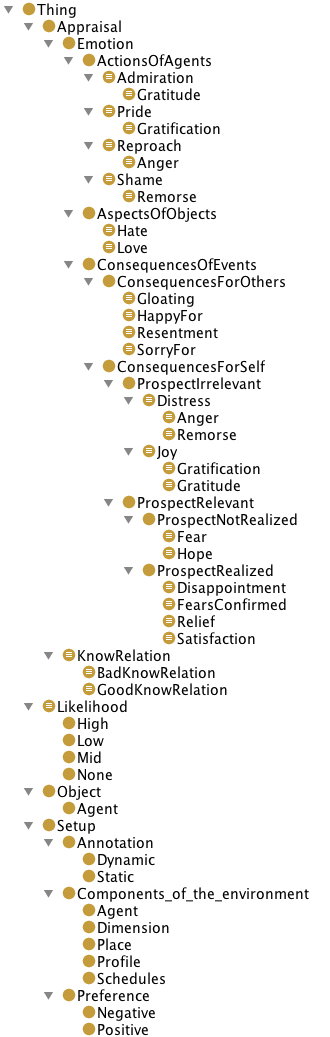
\includegraphics[height=15cm]{figuras/occ_todos_classes.png}
  \caption{Taxonomia das 3 ontologias.}
  \label{fig:tp:cdu:classes}
\end{wrapfigure}

As ontologias explicadas nas seções anteriores foram planejadas para serem
usadas como módulos. Sendo assim, umas das ontologias explicadas anteriormente
pode ser usada sem o uso das demais ou todas em conjunto. Para fins de
exemplificação, nessa seção será utilizada uma ontologia que faz a importação
das três ontologias explicadas anteriormente nesse capítulo.

Os dados das ontologias se encontram resumidos na
Tabela~\ref{tab:tp:cdu:geral}. As
Figuras~\ref{fig:tp:cdu:classes}~e~\ref{fig:tp:cdu:relations} demonstram,
respectivamente, todos os conceitos e todas as relações desenvolvidas durante
o presente trabalho. Além disso, a Figura~\ref{fig:tp:cdu:geral} serve para
demonstrar a importação realizada e comprovar os dados fornecidos.

Os dois primeiros exemplos que serão dados são de erros possíveis na
ontologia. O primeiro exemplo a ser dado é o de uma avaliação que só
possui a relação de probabilidade indo para um indivíduo de conceito. No
exemplo a relação irá para um indivíduo da classe \emph{Low} e essa avaliação
é criada sobre o conceito \emph{Thing}. Como só possui uma única relação não é
possível realizar nenhum outro enquadramento dentro dos conceitos propostos,
note que se a relação de probabilidade tivesse um domínio esse indivíduo
criado seria posto lá e isso pode não ser desejado.

O segundo exemplo é o de uma avaliação de um personagem chamado Dolores. Esse
personagem tem vergonha de sua mãe. Assim, esse indivíduo é configurado
conforme a Figura~\ref{fig:tp:cdu:shameOtherDontSupported}~(a).
Esse exemplo, como dito anteriormente, tem a avaliação sendo considerada de
reprovamento porque no modelo proposto não é possível sentir vergonha por
outra pessoa conforme demostrado na
Figura~\ref{fig:tp:cdu:shameOtherDontSupported}~(b). Entretanto, se a pessoa
tentar forçar a relação \emph{hasJudgeMyself} ao invés da \emph{hasJudge} a
ontologia ficará inconsistente. Note ainda que a avaliação será classificado
como pertence ao conceito \emph{ActionsOfAgents} se não for informado que
Dolores e MaeDolores são indivíduos diferentes. Isso é demostrado na
Figura~\ref{fig:tp:cdu:shameOtherDontSupported}~(c).

\begin{figure}[ht]
    \centering
	\begin{minipage}[t]{\linewidth}
		\centering
	    \begin{tabular}{cc}
		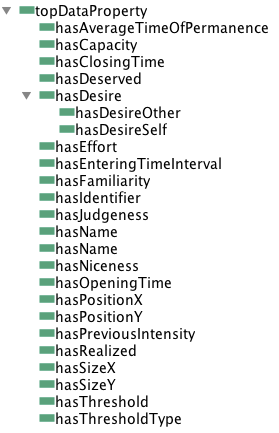
\includegraphics[height=8cm]{figuras/occ_todos_dph.png} \hspace{1cm} & 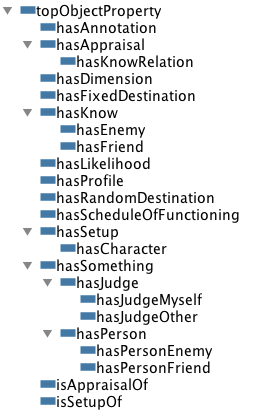
\includegraphics[height=8cm]{figuras/occ_todos_oph.png} \\
	    (i) Relações de dados & (ii) Relações de Objetos
	    \end{tabular}
		\caption{As relações existentes em todas as ontologias.}
		\label{fig:tp:cdu:relations}
	\end{minipage} \vspace{0.3cm} \\
	\begin{minipage}[b]{\linewidth}
		\centering
		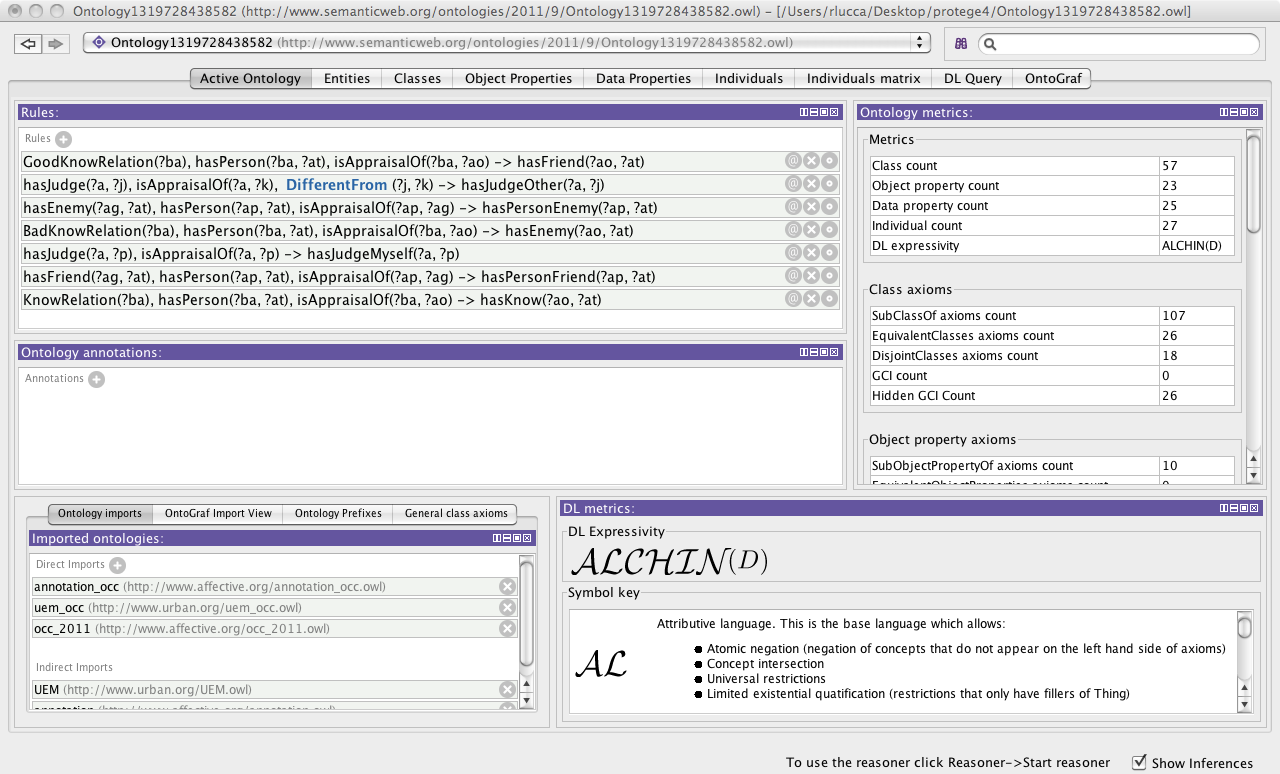
\includegraphics[width=14cm]{figuras/occ_todos_geral.png}
		\caption{Protege 4 mostrando as importações, dados gerais e regras.}
		\label{fig:tp:cdu:geral}
	\end{minipage}
\end{figure}

Os exemplos seguintes são baseados em um cenário especifico. Esse possui
%quatro agentes diferentes: Dilu, John, Jose e Millie. Os perfis desses agentes
dois agentes diferentes: John e Jose. Os perfis desses agentes
%são, respectivamente, \emph{Dependent}, \emph{UnemployedAdult} e os dois
são, respectivamente, \emph{UnemployedAdult} e \emph{EmployedAdult}.
%últimos \emph{EmployedAdult}.
Conforme explicado na seção~\ref{cap:eda:odhv} na página~\pageref{ex:tipos},
%o tipo \emph{Dependent} precisa de um adulto para se mover,
o tipo \emph{UnemployedAdult} possui destinos randômicos somente e
\emph{EmployedAdult} possui destino fixo (o local de trabalho) e alguns
randômicos. Entretanto, a configuração dos locais possíveis foi ignorada
porque só faz sentido descreve-los quando se esta usando a ontologia
dentro de uma aplicação e aqui se esta preocupado em demonstra-la de maneira
isolada.

\begin{figure}[ht]
    \centering
	\begin{minipage}{1.0\linewidth}
	  \centering
	  \begin{tabular}{m{8.5cm}c}
	    \begin{minipage}{\linewidth}
			\centering
			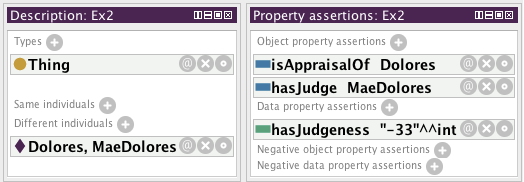
\includegraphics[width=8cm]{figuras/doloresConfig.png} \\
			(a) Configuração da avaliação do agente Dolores sobre sua mãe.
		\end{minipage} &
	    \begin{minipage}{0.40\linewidth}
			\centering
			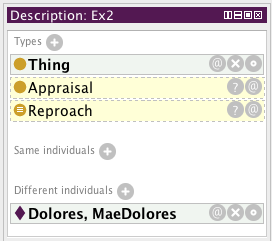
\includegraphics[height=2cm]{figuras/doloresInferencia2.png} \\
				(b) Esperado era a emoção de \emph{Shame} \vspace{0.5cm}\\
			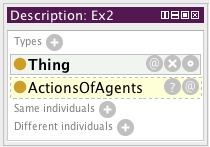
\includegraphics[height=2cm]{figuras/doloresInferencia1.png} \\
				(c) Nenhum conceito de emoção foi inferido
		\end{minipage}
	  \end{tabular}
	\end{minipage}
	\caption{Exemplo com o agente Dolores e seus resultados.}
	\label{fig:tp:cdu:shameOtherDontSupported}
\end{figure}


A Figura~\ref{fig:tp:cdu:johnHasFriendJose} mostra em (a) a configuração
existente na avaliação feita pelo personagem John sobre Jose. Em (b) é
mostrado que o mecanismo de inferência conseguiu definir a avaliação como uma
boa relação. Entretanto, cabe salientar que Jose pode ter outra opinião sobre
John por que amizade não é uma relação simétrica. A
Figura~\ref{fig:tp:cdu:joseHasEnemyJohn} é a avaliação que Jose faz de John
que serve para demonstrar isso. %Além disso, a
%Figura~\ref{fig:tp:cdu:ex9preparo} serve para demonstrar um personagem chamado
%Dilu avaliando Jose.

\begin{figure}[ht]
  \centering
  \begin{tabular}{cc}
  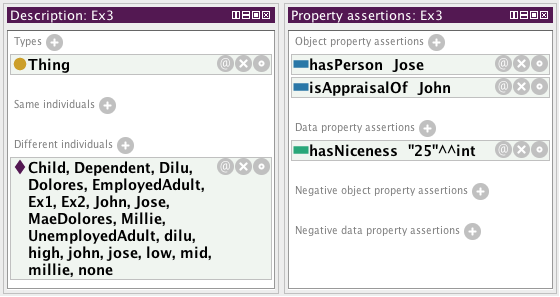
\includegraphics[height=3.5cm]{figuras/appraisalEx3.png} & 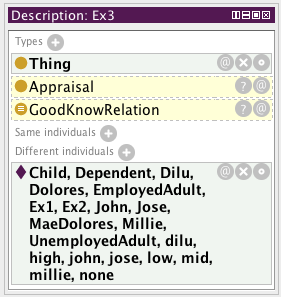
\includegraphics[height=3.5cm]{figuras/infEx3.png} \\
  (a) Configuração & (b) Resultado
  \end{tabular}
  \caption{Avaliação de John sobre Jose.}
  \label{fig:tp:cdu:johnHasFriendJose}
\end{figure}

\begin{figure}[ht]
  \centering
  \begin{tabular}{cc}
  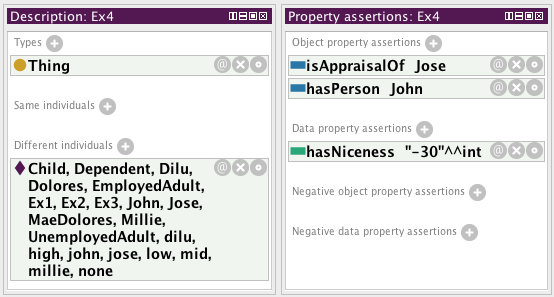
\includegraphics[height=3.5cm]{figuras/appraisalEx4.png} & 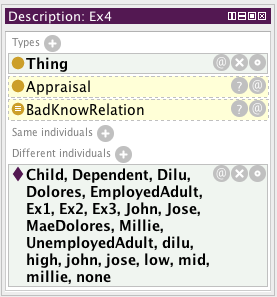
\includegraphics[height=3.5cm]{figuras/infEx4.png} \\
  (a) Configuração & (b) Resultado
  \end{tabular}
  \caption{Avaliação de Jose sobre John.}
  \label{fig:tp:cdu:joseHasEnemyJohn}
\end{figure}

%\vfill

%\begin{figure}
%  \centering
%  \begin{tabular}{cc}
%  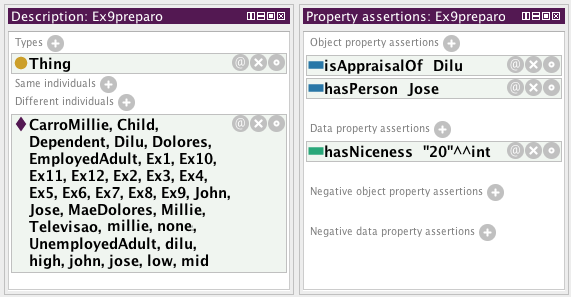
\includegraphics[height=3.5cm]{figuras/appraisalEx9preparo.png} & 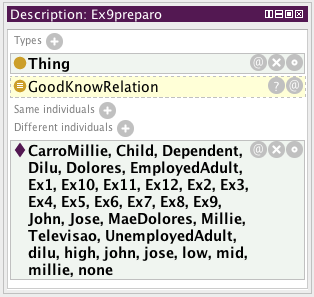
\includegraphics[height=3.5cm]{figuras/infEx9preparo.png} \\
%  (a) Configuração & (b) Resultado
%  \end{tabular}
%  \caption{Avaliação de Dilu sobre Jose.}
%  \label{fig:tp:cdu:ex9preparo}
%\end{figure}

O próximo exemplo, é o da emoção de ódio (\emph{Hate}), serve para demonstrar
que níveis diferentes de intensidade em uma emoção podem ser pensadas como
outras emoções. O personagem John repudia a mídia televisiva, essa
representação é possível de duas formas. A primeira, sendo utilizada na
Figura~\ref{fig:tp:cdu:ex6}, é construir uma avaliação e considerar que o
objeto ``Televisão'' representa toda a mídia televisiva. Sendo assim,
não é possível modelar uma pessoa que não gosta desse tipo de mídia e assiste
noticiários porque seria uma contradição.

A utilização de preferências é a segunda maneira de modelar o personagem John.
Assim, ele pode ter uma preferência negativa contra o objeto de nome
``Televisão''. Entretanto, isso até aqui não é diferente da primeira maneira.
Agora, pense que esse personagem tem uma preferência positiva quando a
utilidade é ``Noticias'' e que esse valor sobrepõem o anterior. Dessa forma, o
agente John pode repudiar a mídia televisiva e assistir um noticiário.

\begin{figure}
  \centering
  \begin{tabular}{cc}
  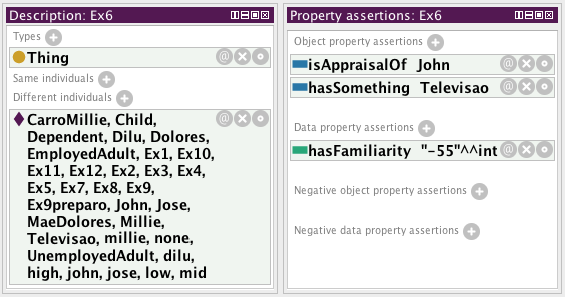
\includegraphics[height=4cm]{figuras/appraisalEx6.png} & 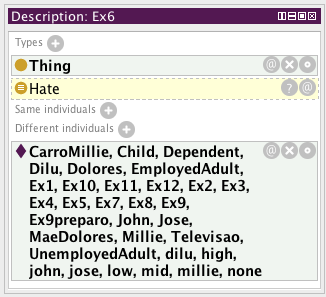
\includegraphics[height=4cm]{figuras/infEx6.png} \\
  (a) Configuração & (b) Resultado
  \end{tabular}
  \caption{Avaliação de repudio de John sobre televisão.}
  \label{fig:tp:cdu:ex6}
\end{figure}


%\newpage
%xxx
%\newpage % 297 de altura e tudo no x acho q nao passo de 815
%\begin{figure}
%  \centering
%  \begin{tabular}{cc}
%  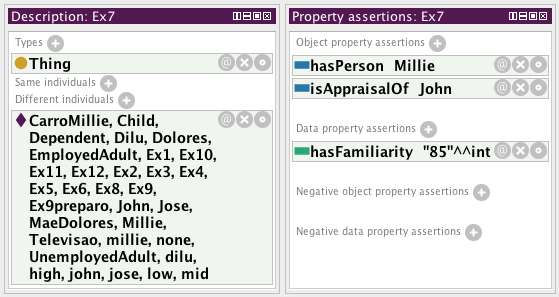
\includegraphics[height=4cm]{figuras/appraisalEx7.png} & 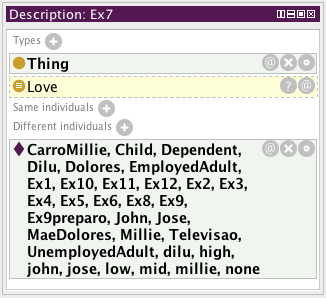
\includegraphics[height=4cm]{figuras/infEx7.png} \\
%  (a) Configuração & (b) Resultado
%  \end{tabular}
%  \caption{Avaliação ...}
%  \label{fig:tp:cdu:ex7}
%\end{figure}
%
%\begin{figure}
%  \centering
%  \begin{tabular}{cc}
%  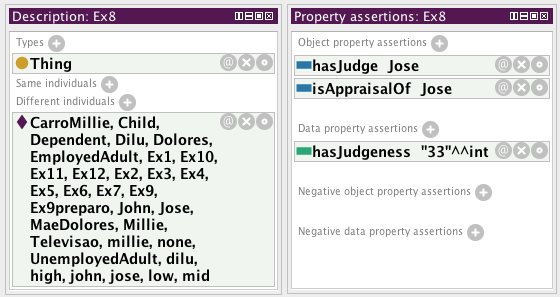
\includegraphics[height=4cm]{figuras/appraisalEx8.png} & 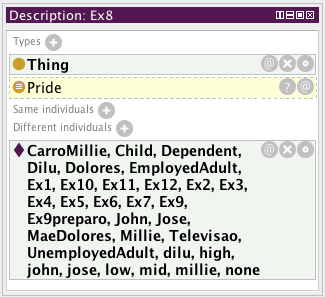
\includegraphics[height=4cm]{figuras/infEx8.png} \\
%  (a) Configuração & (b) Resultado
%  \end{tabular}
%  \caption{Avaliação ...}
%  \label{fig:tp:cdu:ex8}
%\end{figure}
%
%\begin{figure}
%  \centering
%  \begin{tabular}{cc}
%  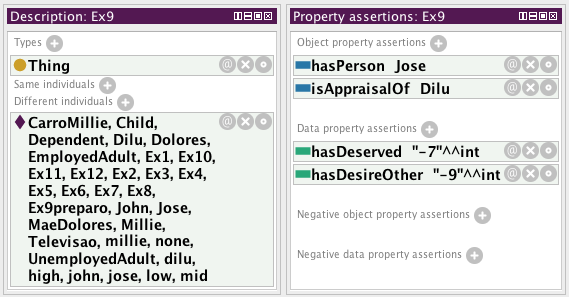
\includegraphics[height=4cm]{figuras/appraisalEx9.png} & 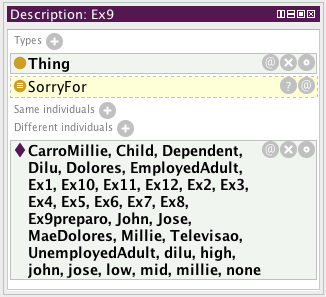
\includegraphics[height=4cm]{figuras/infEx9.png} \\
%  (a) Configuração & (b) Resultado
%  \end{tabular}
%  \caption{Avaliação ...}
%  \label{fig:tp:cdu:ex9}
%\end{figure}
%
%\begin{figure}
%  \centering
%  \begin{tabular}{cc}
%  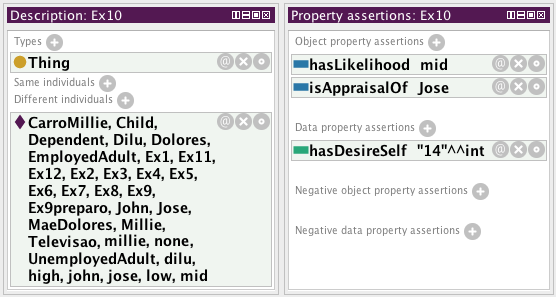
\includegraphics[height=4cm]{figuras/appraisalEx10.png} & 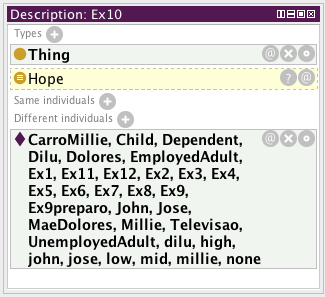
\includegraphics[height=4cm]{figuras/infEx10.png} \\
%  (a) Configuração & (b) Resultado
%  \end{tabular}
%  \caption{Avaliação ...}
%  \label{fig:tp:cdu:ex10}
%\end{figure}
%
%\begin{figure}
%  \centering
%  \begin{tabular}{cc}
%  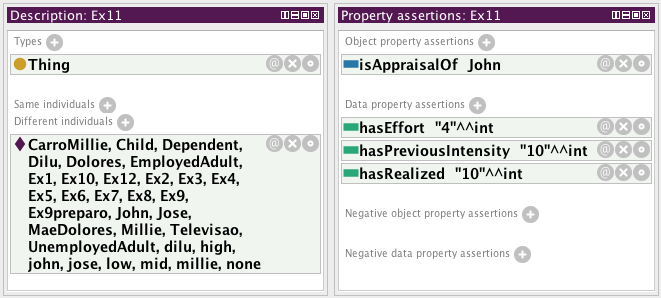
\includegraphics[height=4cm]{figuras/appraisalEx11.png} & 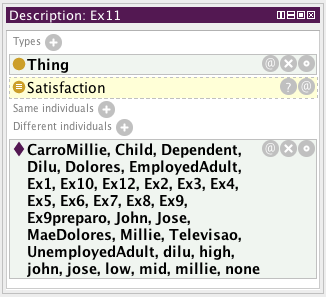
\includegraphics[height=4cm]{figuras/infEx11.png} \\
%  (a) Configuração & (b) Resultado
%  \end{tabular}
%  \caption{Avaliação ...}
%  \label{fig:tp:cdu:ex11}
%\end{figure}
%
%\begin{figure}
%  \centering
%  \begin{tabular}{cc}
%  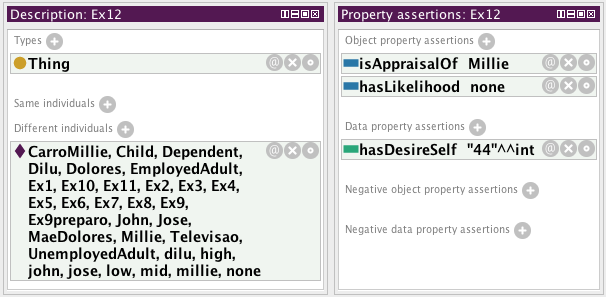
\includegraphics[height=4cm]{figuras/appraisalEx12.png} & 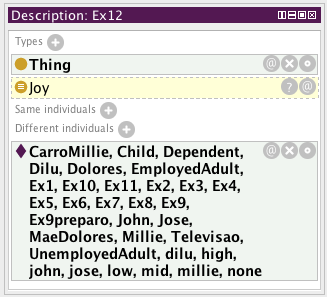
\includegraphics[height=4cm]{figuras/infEx12.png} \\
%  (a) Configuração & (b) Resultado
%  \end{tabular}
%  \caption{Avaliação ...}
%  \label{fig:tp:cdu:ex12}
%\end{figure}
%
%%... tem que tomar o conceito Setup para melhor explicar ele!
%%
%Exemplos do doc:
%John - andarilha		Jose - ele trabalha			Millie - ela trabalha			Dilu - dependente
%%
%ex3 john se da bem com jose
%ex4 jose consira mal john
%ex5 millie julga bem seu carro.
%ex6 john repudia televisao.
%ex7 john gosta/familiar a millie.
%ex8 jose possui orgulho.
%ex9 dilu tem pena de jose.
%	ex9preparo dilu tem boa relacao com jose. (sem isso eh so uma avaliacao e nao SorryFor)
%ex10 Jose tem esperança.
%ex11 John tem satisfação.
%ex12 Millie esta alegre.

